\documentclass{beamer}

\usepackage{amsmath}
\mode<presentation>{\usetheme{UdeA}}
\usepackage[style=verbose]{biblatex}
\addbibresource{biblio.bib}

\usepackage{multimedia}
\usepackage{hyperref}

\renewcommand{\figurename}{Figura}

% Temas de interés: CambridgeUS, Madrid, PaloAlto

\title{Beamer Presentation}
\author{Seminario Investigación\\Facultad de Ingeniería}

\begin{document}
	
	\frame[plain]{\titlepage}
	
	\section{Motivation}
	
	\begin{frame}{Problem Statement}
Definición del problema.


	
	\begin{columns}
		\begin{column}{0.45\linewidth}
			\begin{block}{Definition}
				\begin{figure}
				
\includegraphics[width=0.5\linewidth]{logos/logoUdeA}
				\caption{XXXXXXXXXXX}
			\end{figure}
			\end{block}
		\end{column}
	\begin{column}{0.45\linewidth}
		\begin{figure}
			
\includegraphics[width=0.5\linewidth]{logos/logoUdeA}
			\caption{XXXXXXXXXXX}
		\end{figure}
	\end{column}
	\end{columns}

\begin{columns}
	\begin{column}{0.45\linewidth}
		\begin{block}{Definition}
			\begin{figure}
				
\includegraphics[width=0.5\linewidth]{logos/logoUdeA}
				\caption{XXXXXXXXXXX}
			\end{figure}
		\end{block}
	\end{column}
	\begin{column}{0.45\linewidth}
		\begin{figure}
			
\includegraphics[width=0.5\linewidth]{logos/logoUdeA}
			\caption{XXXXXXXXXXX}
		\end{figure}
	\end{column}
\end{columns}

\end{frame}

\begin{frame}{Test Branch}
HOLA MUNDO! \citeauthor{Rasmunssen05}
\end{frame}
	
	\section{Materials and Methods}
	
	\begin{frame}{PCA}
	\begin{align}
	\mathbf{z} = \mathbf{W}\mathbf{x} 
	\end{align}
	Hola Mundo \footcite{Rasmunssen05}
\end{frame}

\section{Media Files}

\begin{frame}{Video on the computer}
\centering
\movie[externalviewer]{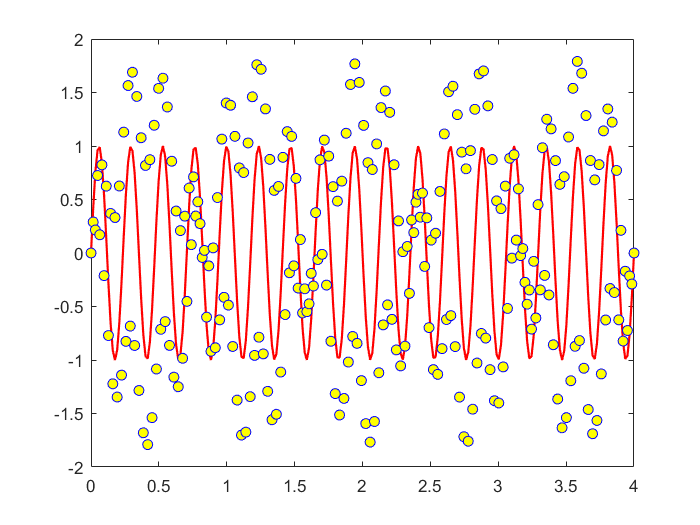
\includegraphics[width=\textheight, keepaspectratio]{img/img2}}{img/sample5s}
\end{frame}

\begin{frame}{YouTube Video}
\begin{figure}
\centering
\href{https://youtu.be/3BLYxQKv668}{
	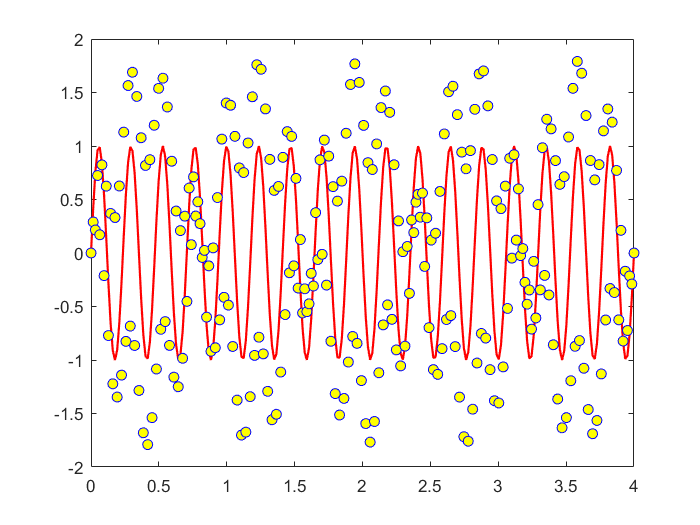
\includegraphics[width=\textheight, keepaspectratio]{img/img2}
	\label{fig:my_label}}
\end{figure}
\end{frame}

	\section{Results}
	
	\begin{frame}{Values}
	\begin{alertblock}{block title}
ALERT BLOCK
	\end{alertblock}
\end{frame}
	\section{Conclusions and Future Works}
	
	\begin{frame}{Conclusions and Future Works}
\begin{itemize}
	\item Conlusion 1
	\begin{itemize}
		\item sub conclusion
	\end{itemize}
\end{itemize}
\end{frame}

\begin{frame}{REF}
%\bibliography{biblio}
%\bibliographystyle{plain}
\printbibliography
\end{frame}

\end{document}
